\chapter{Editor de gramáticas}

El editor de gramáticas es el componente central de SimAS 3.0, diseñado para facilitar la creación, edición y gestión de gramáticas libres de contexto en formato BNF \cite{bnf}. Este editor proporciona un entorno intuitivo y guiado que permite a los usuarios, desde principiantes hasta expertos, crear gramáticas complejas de manera eficiente y sin errores.

\section{Introducción al editor}

El editor de gramáticas de SimAS 3.0 está construido sobre principios de usabilidad y pedagogía, ofreciendo una experiencia de aprendizaje progresiva que guía al usuario a través del proceso de creación de gramáticas mediante un asistente paso a paso.

\subsection{Características principales}

El editor incluye las siguientes características principales:

\begin{itemize}
    \item \textbf{Asistente guiado}: proceso de creación en 4 pasos con validación al finalizar.
    \item \textbf{Validación automática}: verificación de gramáticas cargadas desde archivo y al finalizar el proceso de creación/edición.
    \item \textbf{Validación manual}: el usuario puede validar manualmente al finalizar el proceso de creación/edición.
    \item \textbf{Formato BNF}: soporte completo para el formato de notación Backus-Naur.
    \item \textbf{Interfaz intuitiva}: diseño claro y organizado que facilita la comprensión.
    \item \textbf{Gestión de archivos}: guardado y carga de gramáticas en formato XML.
    \item \textbf{Integración con simulador}: transición directa al simulador para probar la gramática.
\end{itemize}

\subsection{Objetivos del editor}

Los objetivos principales del editor son:

\begin{itemize}
    \item \textbf{Educativo}: proporcionar una herramienta de aprendizaje para estudiantes de informática.
    \item \textbf{Profesional}: ofrecer funcionalidades avanzadas para usuarios experimentados.
    \item \textbf{Validación}: asegurar la corrección sintáctica y semántica de las gramáticas.
    \item \textbf{Eficiencia}: acelerar el proceso de creación y edición de gramáticas.
\end{itemize}

\section{Acceso al editor}

El editor de gramáticas se puede acceder de múltiples maneras desde la interfaz principal de SimAS 3.0.

\subsection{Métodos de acceso}

Para abrir el editor de gramáticas:

\begin{enumerate}
    \item \textbf{Desde el menú principal}: haga clic en el botón \string"Editor de gramáticas\string".
    \item \textbf{Atajo de teclado}: presione \texttt{Ctrl+N} desde cualquier ventana.
\end{enumerate}

\section{Interfaz del editor}

Al abrir el editor, se presenta una interfaz organizada que muestra toda la información relacionada con la gramática actual.

\subsection{Estado vacío del editor}

Cuando se abre el editor por primera vez o no hay ninguna gramática cargada, la interfaz se muestra vacía como se puede ver en la figura \ref{fig:editor_vacio}.

\needspace{8cm}
\begin{figure}[H]
    \centering
    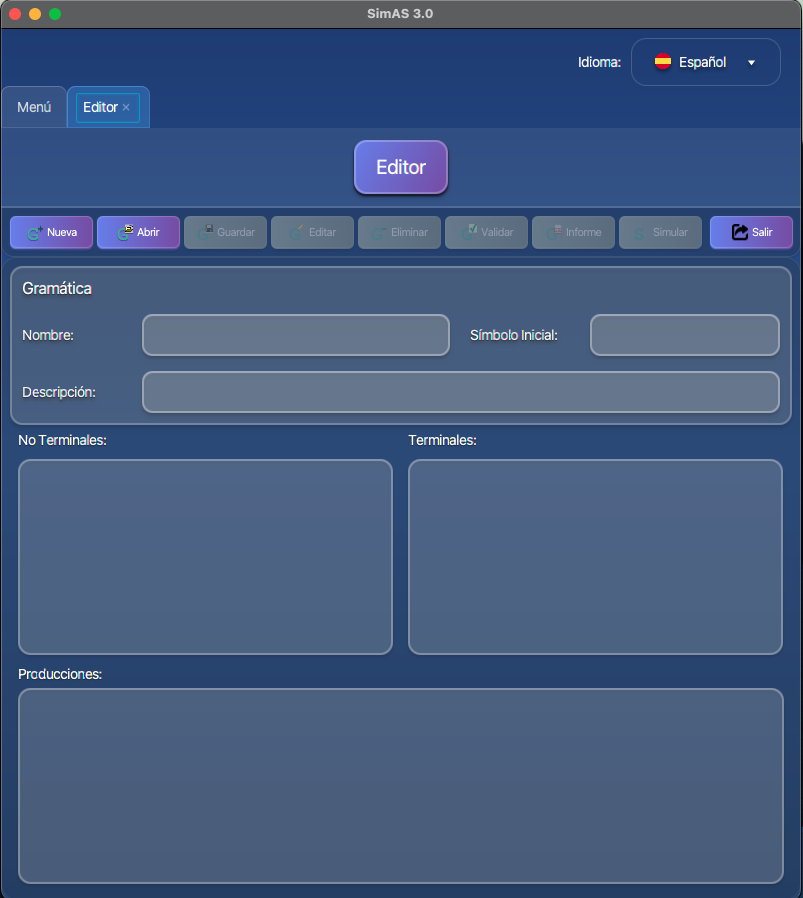
\includegraphics[width=0.9\textwidth]{figuras/editor/editor_vacio.png}
    \caption{Editor de gramáticas en estado vacío}
    \label{fig:editor_vacio}
\end{figure}

En este estado, la interfaz muestra:
\begin{itemize}
    \item \textbf{Barra de herramientas}: con los botones \string"Nueva\string", \string"Abrir\string" y \string"Salir\string" habilitados, y el resto deshabilitados.
    \item \textbf{Área principal}: completamente vacía, lista para mostrar la información de una gramática.
    \item \textbf{Información de la gramática}: campos vacíos para nombre, descripción, símbolos y producciones.
\end{itemize}

\subsection{Estado con gramática cargada}

Cuando se carga una gramática existente, la interfaz se actualiza automáticamente para mostrar toda la información de la gramática, como se muestra en la figura \ref{fig:editor_con_gramatica}.

\needspace{8cm}
\begin{figure}[H]
    \centering
    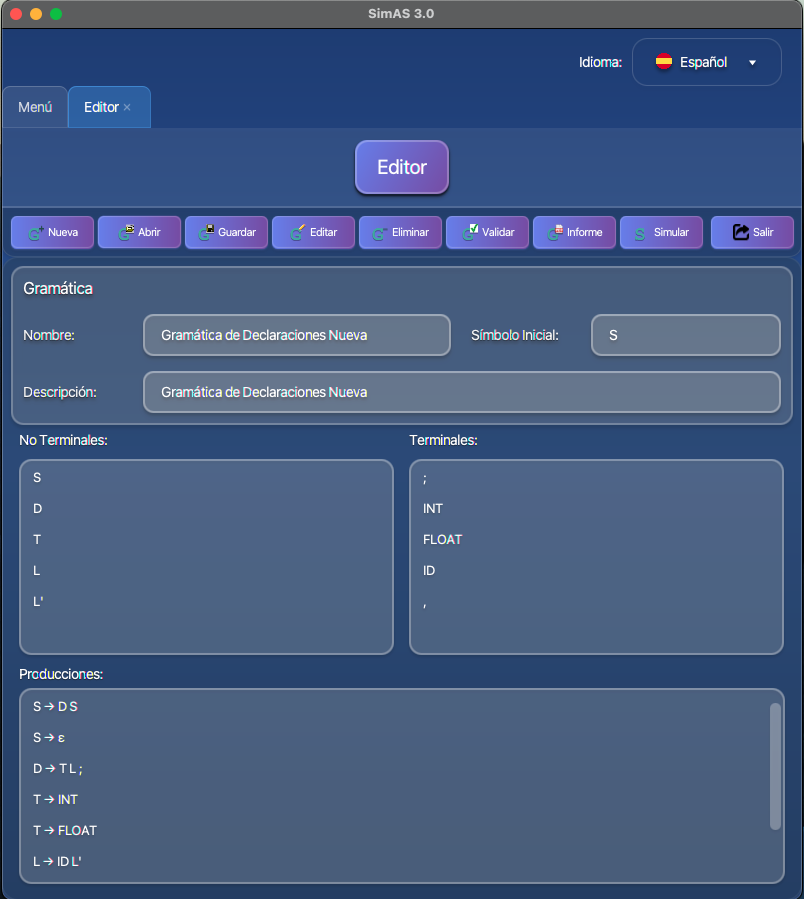
\includegraphics[width=0.9\textwidth]{figuras/editor/editor.png}
    \caption{Editor de gramáticas con una gramática cargada}
    \label{fig:editor_con_gramatica}
\end{figure}

En este estado, la interfaz muestra:
\begin{itemize}
    \item \textbf{Barra de herramientas}: con todos los botones habilitados.
    \item \textbf{Información de la gramática}: nombre, descripción, símbolos terminales, símbolos no terminales y producciones.
\end{itemize}

\subsection{Barra de herramientas}

La barra de herramientas del editor incluye los siguientes botones:

\begin{itemize}
    \item \textbf{Botón \string"Nueva\string"}: abre el asistente de creación para crear una nueva gramática desde cero.
    \item \textbf{Botón \string"Abrir\string"}: carga una gramática existente desde un archivo XML.
    \item \textbf{Botón \string"Guardar\string"}: guarda la gramática actual en un archivo XML (solo disponible cuando hay una gramática cargada).
    \item \textbf{Botón \string"Editar\string"}: abre el asistente de edición con la gramática actual cargada (solo disponible cuando hay una gramática cargada).
    \item \textbf{Botón \string"Eliminar\string"}: elimina la gramática actual del editor (solo disponible cuando hay una gramática cargada).
    \item \textbf{Botón \string"Validar\string"}: ejecuta la validación de la gramática actual (solo disponible cuando hay una gramática cargada).
    \item \textbf{Botón \string"Informe\string"}: genera un informe detallado de la gramática actual (solo disponible cuando hay una gramática cargada).
    \item \textbf{Botón \string"Simular\string"}: transfiere la gramática al simulador para su análisis (solo disponible cuando hay una gramática cargada).
    \item \textbf{Botón \string"Salir\string"}: cierra la aplicación.
\end{itemize}

\section{Asistente guiado de creación}

El asistente guiado es una de las características más destacadas del editor, diseñado para simplificar el proceso de creación y edición de gramáticas mediante un enfoque paso a paso.

\subsection{Acceso al asistente}

El asistente se puede abrir de dos maneras:

\begin{itemize}
    \item \textbf{Botón \string"Nueva\string"}: abre el asistente vacío para crear una nueva gramática desde cero.
    \item \textbf{Botón \string"Editar\string"}: abre el asistente con la gramática actual cargada para editarla (solo disponible cuando hay una gramática cargada).
\end{itemize}

\subsection{Proceso de creación}

El asistente divide la creación/edición de gramáticas en cuatro pasos lógicos:

\begin{enumerate}
    \item \textbf{Paso 1 - Datos}: definición del nombre y descripción de la gramática.
    \item \textbf{Paso 2 - Símbolos}: definición de símbolos terminales y no terminales.
    \item \textbf{Paso 3 - Producciones}: creación de las reglas de producción.
    \item \textbf{Paso 4 - Inicial}: selección del símbolo inicial y finalización.
\end{enumerate}

\subsection{Navegación del asistente}

El asistente incluye un menú inferior que permite:

\begin{itemize}
    \item \textbf{Navegación entre pasos}: avanzar y retroceder entre los diferentes pasos.
    \item \textbf{Validación de pasos}: no se permite continuar al siguiente paso si el actual está vacío.
    \item \textbf{Finalización}: al completar el paso 4, los cambios se reflejan en el editor principal.
\end{itemize}

\subsection{Paso 1: Datos de la gramática}

En el primer paso, el usuario define los datos básicos de la gramática: nombre y descripción.

\subsubsection{Interfaz del paso 1}

La interfaz del paso 1 se muestra en la figura \ref{fig:paso1_datos}.

\needspace{8cm}
\begin{figure}[H]
    \centering
    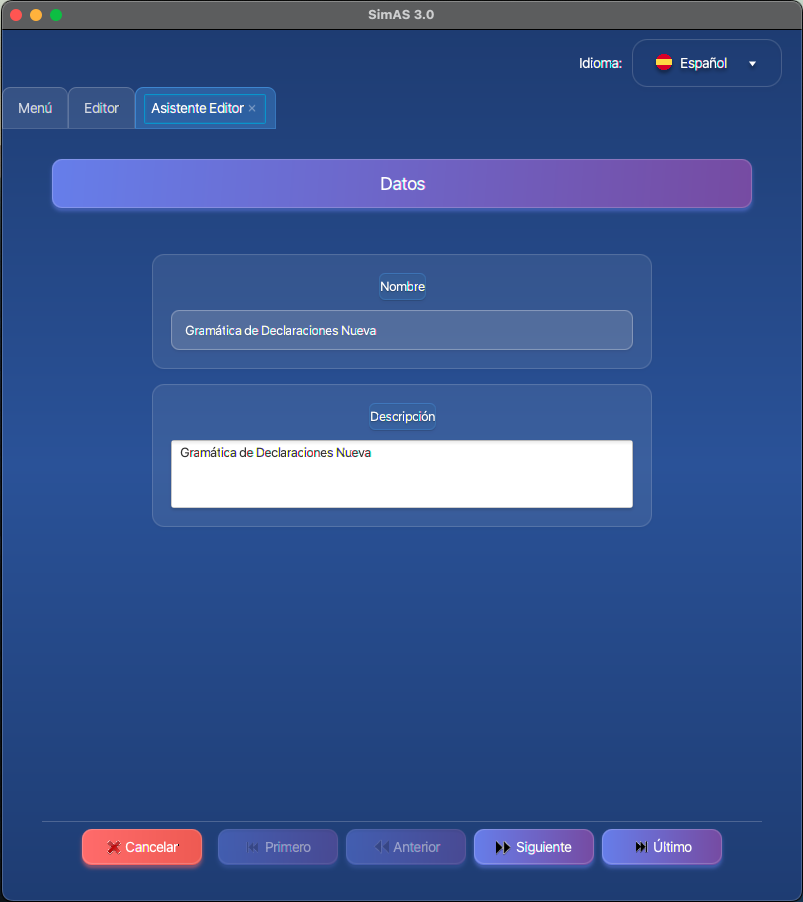
\includegraphics[width=0.9\textwidth]{figuras/editor/paso1_datos.png}
    \caption{Paso 1: Datos de la gramática}
    \label{fig:paso1_datos}
\end{figure}

\subsubsection{Campos del paso 1}

El paso 1 incluye los siguientes campos:

\begin{itemize}
    \item \textbf{Nombre de la gramática}: campo de texto para introducir el nombre que identificará la gramática.
    \item \textbf{Descripción}: campo de texto para proporcionar una descripción detallada de la gramática.
\end{itemize}

\subsubsection{Estado vacío del paso 1}

Si el paso 1 está vacío, se muestra la interfaz de la figura \ref{fig:paso1_vacio} y no se permite continuar al siguiente paso.

\needspace{8cm}
\begin{figure}[H]
    \centering
    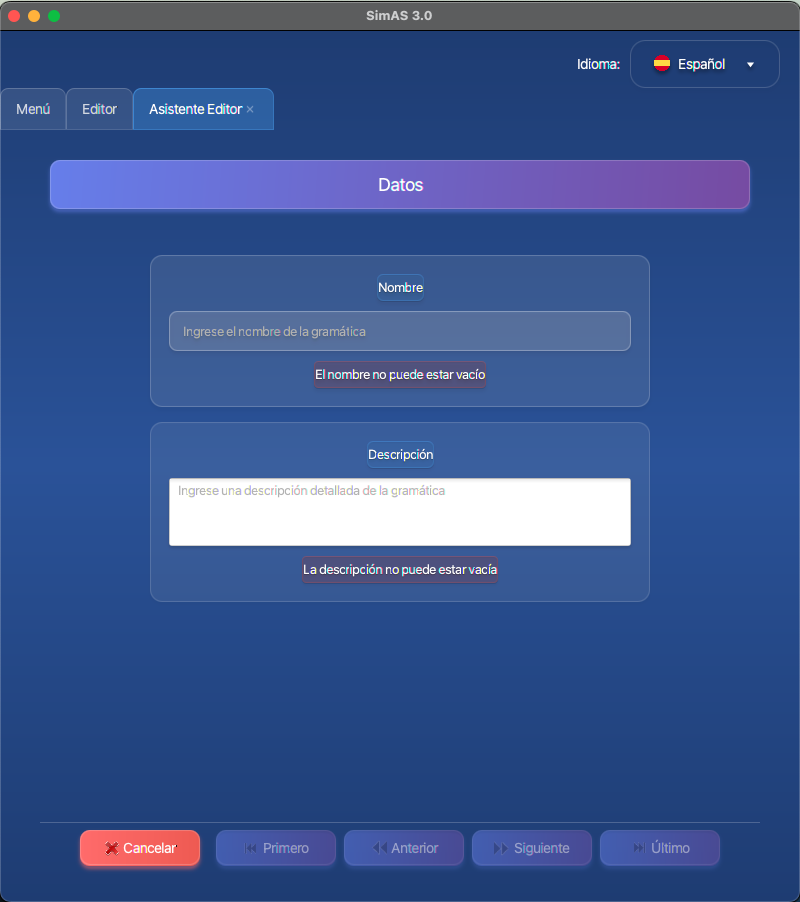
\includegraphics[width=0.9\textwidth]{figuras/editor/paso1_datos_vacio.png}
    \caption{Paso 1: Estado vacío}
    \label{fig:paso1_vacio}
\end{figure}

\subsubsection{Requisitos del paso 1}

Para poder continuar al paso 2, es necesario:

\begin{itemize}
    \item \textbf{Nombre obligatorio}: el campo nombre debe estar rellenado.
    \item \textbf{Descripción obligatorio}: el campo descripción debe estar rellenado.
\end{itemize}

\subsection{Paso 2: Símbolos}

En el segundo paso, el usuario define tanto los símbolos terminales como los no terminales de la gramática.

\subsubsection{Interfaz del paso 2}

La interfaz del paso 2 se muestra en la figura \ref{fig:paso2_simbolos}.

\needspace{8cm}
\begin{figure}[H]
    \centering
    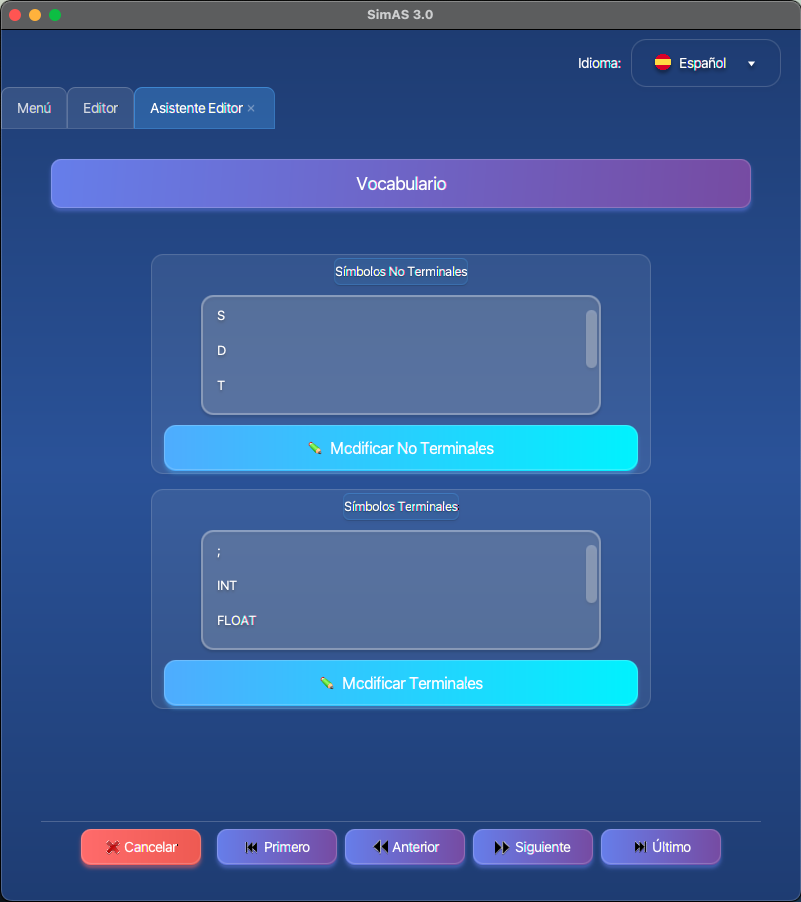
\includegraphics[width=0.9\textwidth]{figuras/editor/paso2_simbolos.png}
    \caption{Paso 2: Símbolos de la gramática}
    \label{fig:paso2_simbolos}
\end{figure}

\subsubsection{Estado vacío del paso 2}

Si el paso 2 está vacío, se muestra la interfaz de la figura \ref{fig:paso2_vacio} y no se permite continuar al siguiente paso.

\needspace{8cm}
\begin{figure}[H]
    \centering
    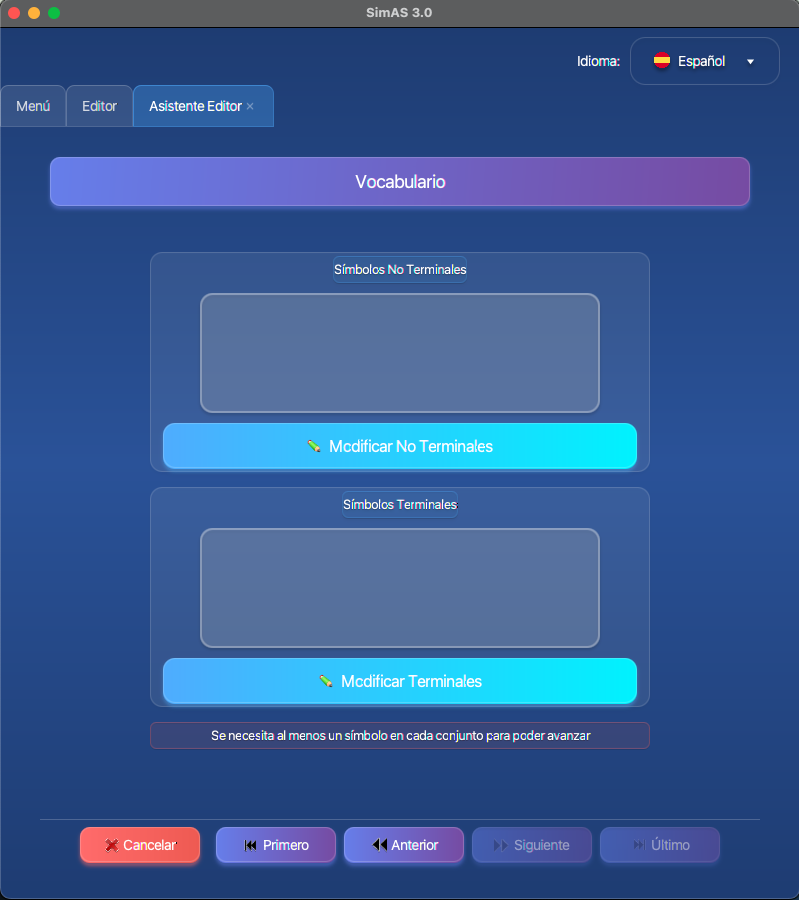
\includegraphics[width=0.9\textwidth]{figuras/editor/paso2_simbolos_vacio.png}
    \caption{Paso 2: Estado vacío}
    \label{fig:paso2_vacio}
\end{figure}

\subsubsection{Elementos del paso 2}

El paso 2 incluye los siguientes elementos:

\begin{itemize}
    \item \textbf{Lista de símbolos terminales}: muestra todos los símbolos terminales definidos.
    \item \textbf{Lista de símbolos no terminales}: muestra todos los símbolos no terminales definidos.
    \item \textbf{Botón \string"Modificar símbolos terminales\string"}: abre el panel auxiliar para gestionar símbolos terminales.
    \item \textbf{Botón \string"Modificar símbolos no terminales\string"}: abre el panel auxiliar para gestionar símbolos no terminales.
    \item \textbf{Indicador de estado}: muestra si el paso está incompleto.
\end{itemize}

\subsubsection{Paneles auxiliares}

El paso 2 permite abrir dos paneles auxiliares para la gestión de símbolos:

\begin{itemize}
    \item \textbf{Panel de símbolos terminales}: para insertar, editar o eliminar símbolos terminales.
    \item \textbf{Panel de símbolos no terminales}: para insertar, editar o eliminar símbolos no terminales.
\end{itemize}

\subsubsection{Panel de símbolos terminales}

Al hacer clic en el botón correspondiente, se abre el panel de símbolos terminales mostrado en la figura \ref{fig:panel_terminales}.

\needspace{8cm}
\begin{figure}[H]
    \centering
    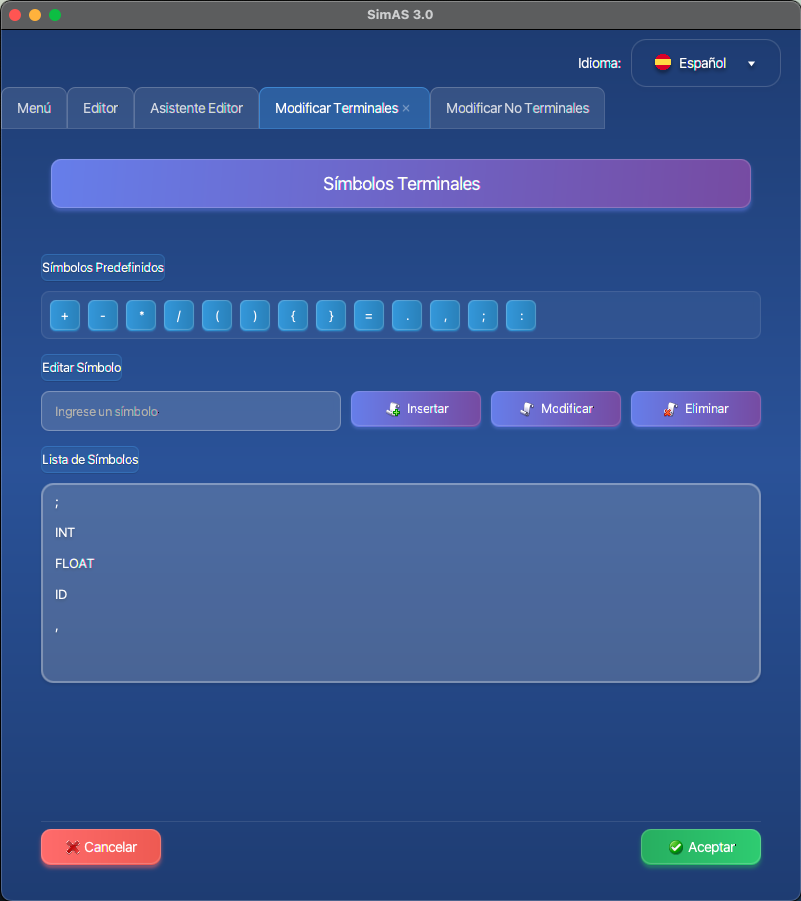
\includegraphics[width=0.9\textwidth]{figuras/editor/panel_terminales.png}
    \caption{Panel de símbolos terminales}
    \label{fig:panel_terminales}
\end{figure}

\subsubsection{Elementos del panel de símbolos terminales}

Este panel incluye los siguientes elementos:

\begin{itemize}
    \item \textbf{Símbolos predefinidos}: lista de símbolos comunes que se pueden insertar rápidamente.
    \item \textbf{Campo de texto}: para introducir nuevos símbolos terminales.
    \item \textbf{Botón \string"Insertar\string"}: añade el símbolo del campo de texto a la lista.
    \item \textbf{Botón \string"Modificar\string"}: permite modificar un símbolo seleccionado.
    \item \textbf{Botón \string"Eliminar\string"}: quita el símbolo seleccionado de la lista.
    \item \textbf{Botón \string"Aceptar\string"}: confirma los cambios y cierra el panel.
    \item \textbf{Botón \string"Cancelar\string"}: descarta los cambios y cierra el panel.
\end{itemize}

\subsubsection{Funcionalidades del panel de símbolos terminales}

Este panel permite:
\begin{itemize}
    \item \textbf{Insertar terminales}: introducir nuevos símbolos terminales.
    \item \textbf{Modificar terminales}: editar símbolos terminales existentes.
    \item \textbf{Eliminar terminales}: quitar símbolos terminales de la gramática.
    \item \textbf{Usar símbolos predefinidos}: seleccionar símbolos comunes de una lista.
\end{itemize}

\subsubsection{Panel de símbolos no terminales}

Al hacer clic en el botón correspondiente, se abre el panel de símbolos no terminales mostrado en la figura \ref{fig:panel_no_terminales}.

\needspace{8cm}
\begin{figure}[H]
    \centering
    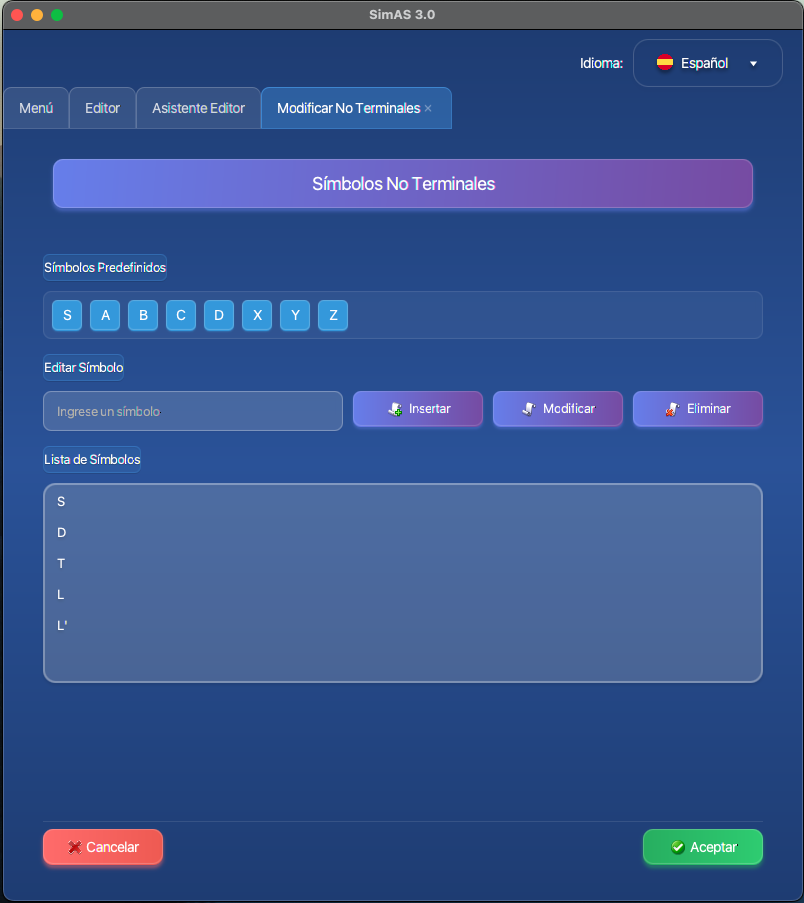
\includegraphics[width=0.9\textwidth]{figuras/editor/panel_no_terminales.png}
    \caption{Panel de símbolos no terminales}
    \label{fig:panel_no_terminales}
\end{figure}

\subsubsection{Elementos del panel de símbolos no terminales}

Este panel incluye los siguientes elementos:

\begin{itemize}
    \item \textbf{Símbolos predefinidos}: lista de símbolos comunes que se pueden insertar rápidamente.
    \item \textbf{Campo de texto}: para introducir nuevos símbolos no terminales.
    \item \textbf{Botón \string"Insertar\string"}: añade el símbolo del campo de texto a la lista.
    \item \textbf{Botón \string"Modificar\string"}: permite editar un símbolo seleccionado.
    \item \textbf{Botón \string"Eliminar\string"}: quita el símbolo seleccionado de la lista.
    \item \textbf{Botón \string"Aceptar\string"}: confirma los cambios y cierra el panel.
    \item \textbf{Botón \string"Cancelar\string"}: descarta los cambios y cierra el panel.
\end{itemize}

\subsubsection{Funcionalidades del panel de símbolos no terminales}

Este panel permite:
\begin{itemize}
    \item \textbf{Insertar no terminales}: introducir nuevos símbolos no terminales.
    \item \textbf{Modificar no terminales}: editar símbolos no terminales existentes.
    \item \textbf{Eliminar no terminales}: quitar símbolos no terminales de la gramática.
    \item \textbf{Usar símbolos predefinidos}: seleccionar símbolos comunes de una lista.
\end{itemize}

\subsubsection{Requisitos del paso 2}

Para poder continuar al paso 3, es necesario:

\begin{itemize}
    \item \textbf{Al menos un símbolo}: debe haber al menos un símbolo terminal y no terminal definido.
    \item \textbf{Símbolos únicos}: no puede haber símbolos duplicados.
\end{itemize}

\subsection{Paso 3: Producciones}

En el tercer paso, el usuario define las reglas de producción que relacionan los símbolos no terminales con secuencias de símbolos.

\subsubsection{Interfaz del paso 3}

La interfaz del paso 3 se muestra en la figura \ref{fig:paso3_producciones}.

\needspace{8cm}
\begin{figure}[H]
    \centering
    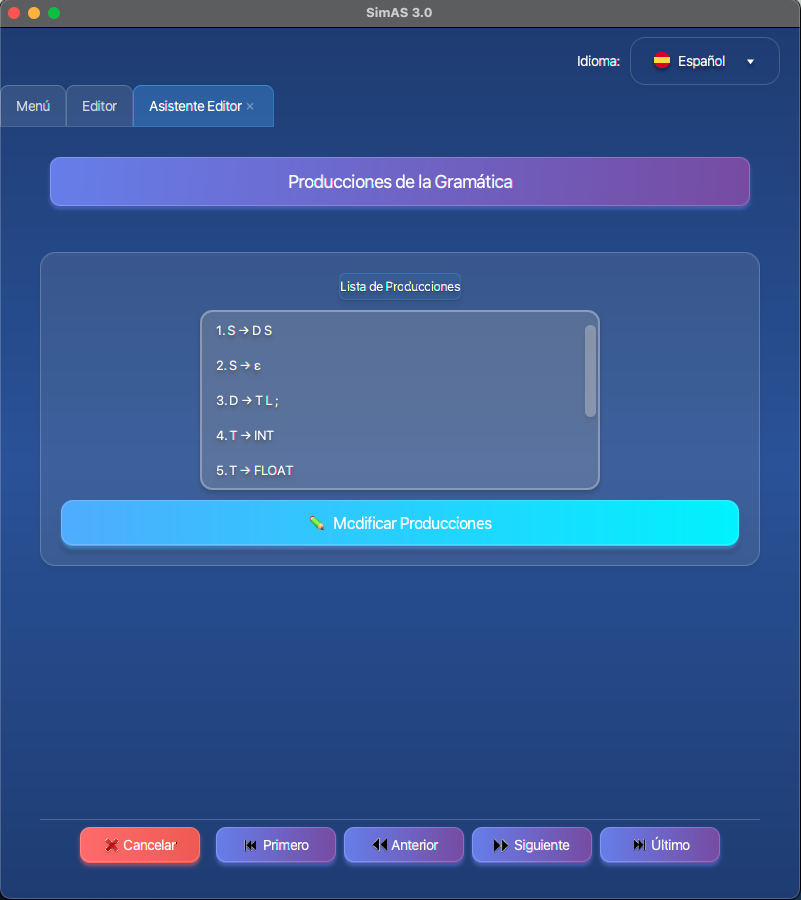
\includegraphics[width=0.9\textwidth]{figuras/editor/paso3_producciones.png}
    \caption{Paso 3: Producciones de la gramática}
    \label{fig:paso3_producciones}
\end{figure}

\subsubsection{Estado vacío del paso 3}

Si el paso 3 está vacío, se muestra la interfaz de la figura \ref{fig:paso3_vacio} y no se permite continuar al siguiente paso.

\needspace{8cm}
\begin{figure}[H]
    \centering
    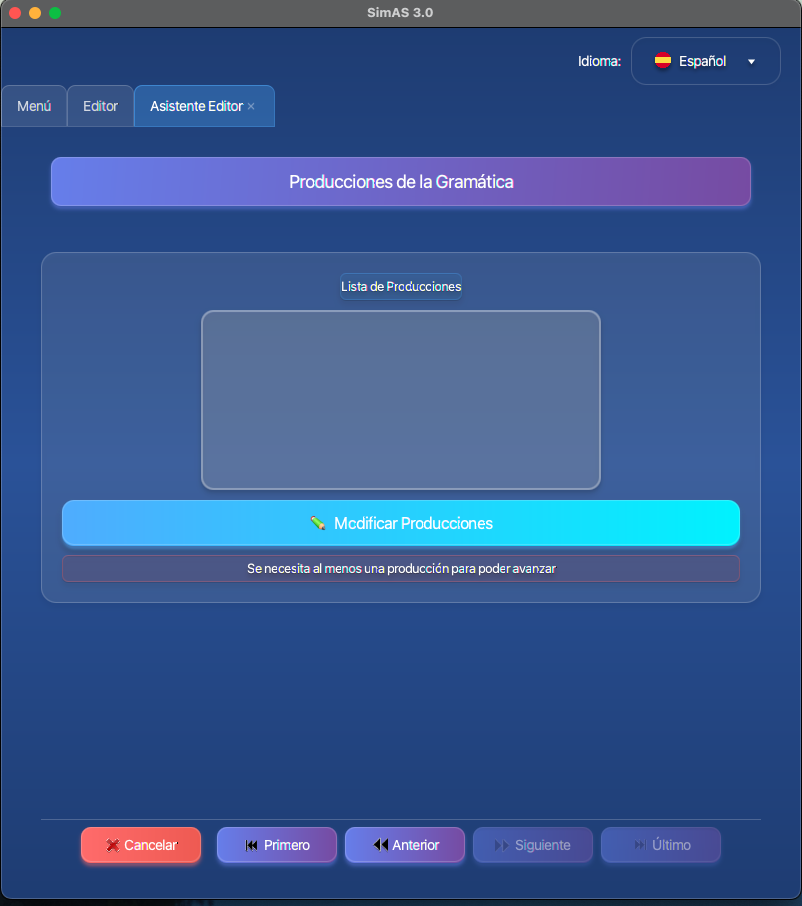
\includegraphics[width=0.9\textwidth]{figuras/editor/paso3_producciones_vacio.png}
    \caption{Paso 3: Estado vacío}
    \label{fig:paso3_vacio}
\end{figure}

\subsubsection{Elementos del paso 3}

El paso 3 incluye los siguientes elementos:

\begin{itemize}
    \item \textbf{Lista de producciones}: muestra todas las reglas de producción definidas.
    \item \textbf{Botón \string"Modificar producciones\string"}: abre el panel auxiliar para gestionar producciones.
    \item \textbf{Indicador de estado}: muestra si el paso está incompleto.
\end{itemize}

\subsubsection{Panel de producciones}

Al hacer clic en el botón correspondiente, se abre el panel de producciones mostrado en la figura \ref{fig:panel_producciones}.

\needspace{8cm}
\begin{figure}[H]
    \centering
    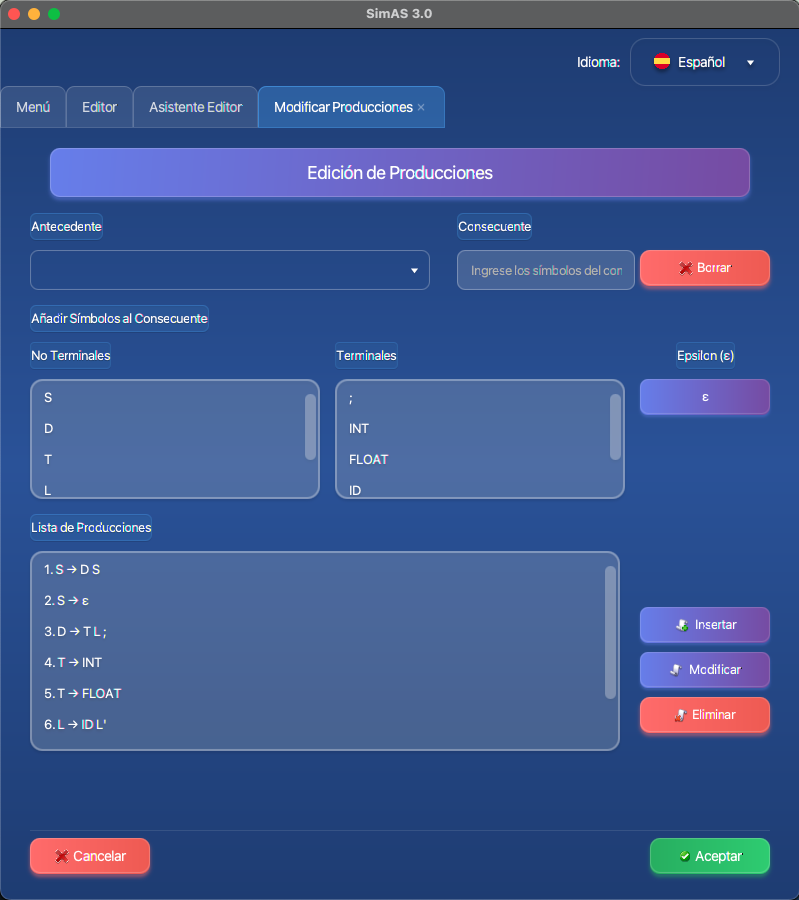
\includegraphics[width=0.9\textwidth]{figuras/editor/panel_producciones.png}
    \caption{Panel de producciones}
    \label{fig:panel_producciones}
\end{figure}

\subsubsection{Elementos del panel de producciones}

Este panel incluye los siguientes elementos:

\begin{itemize}
    \item \textbf{Lista de producciones}: muestra todas las reglas de producción definidas.
    \item \textbf{Selector de símbolo no terminal}: permite elegir el símbolo no terminal (antecedente) para la producción.
    \item \textbf{Editor de consecuente}: área para construir la secuencia de símbolos del consecuente.
    \item \textbf{Lista de símbolos disponibles}: muestra los símbolos terminales y no terminales que se pueden usar.
    \item \textbf{Botón \string"Insertar\string"}: añade la producción construida a la lista.
    \item \textbf{Botón \string"Modificar\string"}: permite editar una producción seleccionada.
    \item \textbf{Botón \string"Eliminar\string"}: quita la producción seleccionada de la lista.
    \item \textbf{Botón \string"Aceptar\string"}: confirma los cambios y cierra el panel.
    \item \textbf{Botón \string"Cancelar\string"}: descarta los cambios y cierra el panel.
    \item \textbf{Vista previa}: muestra cómo se verá la producción en formato BNF.
\end{itemize}

\subsubsection{Funcionalidades del panel de producciones}

Este panel permite:
\begin{itemize}
    \item \textbf{Insertar producciones}: crear nuevas reglas de producción.
    \item \textbf{Modificar producciones}: editar producciones existentes.
    \item \textbf{Eliminar producciones}: quitar producciones de la gramática.
    \item \textbf{Construir consecuentes}: doble clic en los símbolos disponibles para crear secuencias.
    \item \textbf{Vista previa en tiempo real}: ver el formato BNF mientras se construye.
\end{itemize}

\subsubsection{Formato de producciones}

Las producciones siguen el formato estándar BNF:

\begin{itemize}
    \item \textbf{Antecedente}: símbolo no terminal a la izquierda.
    \item \textbf{Flecha}: símbolo \texttt{::=} que indica \string"se define como\string".
    \item \textbf{Consecuente}: secuencia de símbolos a la derecha.
\end{itemize}

\subsubsection{Requisitos del paso 3}

Para poder continuar al paso 4, es necesario:

\begin{itemize}
    \item \textbf{Al menos una producción}: debe haber al menos una regla de producción definida.
    \item \textbf{Producciones válidas}: todas las producciones deben estar bien formadas.
\end{itemize}

\subsection{Paso 4: Símbolo inicial}

En el cuarto paso, el usuario selecciona el símbolo inicial de la gramática y finaliza el proceso de creación/edición.

\subsubsection{Interfaz del paso 4}

La interfaz del paso 4 se muestra en la figura \ref{fig:paso4_inicial}.

\needspace{8cm}
\begin{figure}[H]
    \centering
    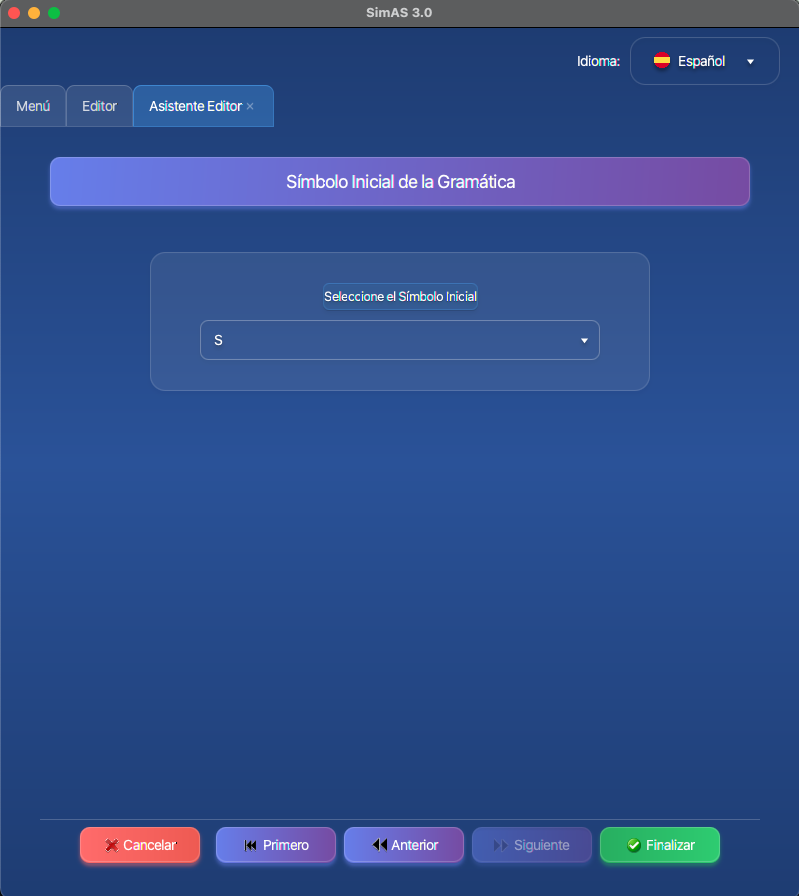
\includegraphics[width=0.9\textwidth]{figuras/editor/paso4_inicial.png}
    \caption{Paso 4: Selección del símbolo inicial}
    \label{fig:paso4_inicial}
\end{figure}

\subsubsection{Estado vacío del paso 4}

Si el paso 4 está vacío, se muestra la interfaz de la figura \ref{fig:paso4_vacio} y no se permite finalizar el proceso.

\needspace{8cm}
\begin{figure}[H]
    \centering
    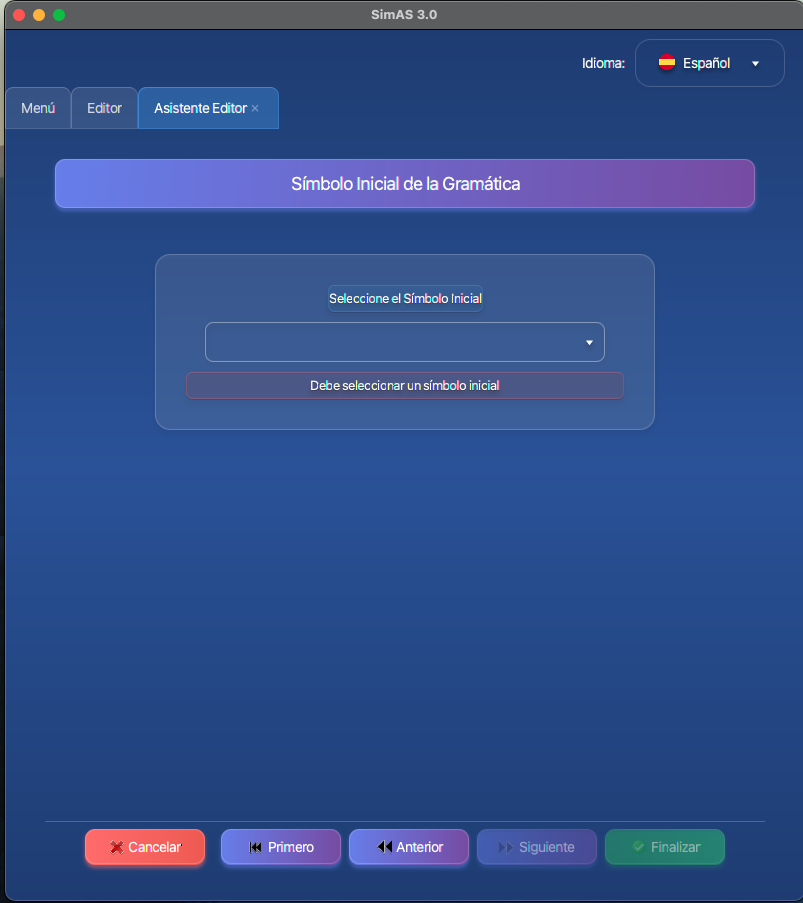
\includegraphics[width=0.9\textwidth]{figuras/editor/paso4_inicial_vacio.png}
    \caption{Paso 4: Estado vacío (no se puede finalizar)}
    \label{fig:paso4_vacio}
\end{figure}

\subsubsection{Selección del símbolo inicial}

En este paso, el usuario debe:

\begin{itemize}
    \item \textbf{Seleccionar símbolo inicial}: elegir uno de los símbolos no terminales definidos como símbolo inicial de la gramática.
    \item \textbf{Finalizar proceso}: al completar la selección, se puede finalizar el proceso.
\end{itemize}

\subsubsection{Finalización del proceso}

Al finalizar el paso 4:

\begin{itemize}
    \item \textbf{Reflejo en el editor}: todos los cambios se reflejan automáticamente en la pestaña del editor principal.
    \item \textbf{Validación automática}: la gramática es validada automáticamente por el sistema.
    \item \textbf{Cierre del asistente}: el asistente se cierra y regresa al editor principal.
\end{itemize}

\section{Gestión de archivos}

El editor incluye un sistema completo de gestión de archivos que permite guardar, cargar y exportar gramáticas.

\subsection{Formato de archivo}

Las gramáticas se guardan en formato XML, que proporciona:

\begin{itemize}
    \item \textbf{Estructura clara}: organización jerárquica de los elementos.
    \item \textbf{Extensibilidad}: facilidad para agregar nuevas características.
    \item \textbf{Compatibilidad}: estándar ampliamente soportado.
    \item \textbf{Legibilidad}: formato que puede ser leído por humanos.
\end{itemize}

\subsection{Operaciones de archivo}

Las operaciones disponibles incluyen:

\begin{itemize}
    \item \textbf{Nuevo}: crear una nueva gramática en blanco.
    \item \textbf{Abrir}: cargar una gramática existente desde el disco.
    \item \textbf{Guardar}: guardar la gramática actual.
    \item \textbf{Eliminar}: eliminar la gramática actual.
    \item \textbf{Validar}: validar la gramática actual.
    \item \textbf{Informe}: generar un informe detallado de la gramática actual.
\end{itemize}

\subsection{Ubicación de archivos}

Los archivos se pueden guardar en:

\begin{itemize}
    \item \textbf{Ubicación personalizada}: el usuario elige dónde guardar.
    \item \textbf{Carpeta de proyectos}: directorio dedicado para gramáticas.
    \item \textbf{Ubicación temporal}: se guarda en el directorio temporal para trabajos en progreso.
    \item \textbf{Ubicación de respaldo}: copias de seguridad generadas por el usuario.
\end{itemize}

\section{Validación de gramáticas}

La validación de gramáticas es un proceso fundamental que asegura la corrección sintáctica y semántica de las gramáticas creadas.

\subsection{Tipos de validación}

El editor realiza dos tipos de validación:

\begin{itemize}
    \item \textbf{Validación automática}: se ejecuta automáticamente cuando se carga una gramática desde archivo.
    \item \textbf{Validación manual}: debe ser ejecutada por el usuario al finalizar el proceso de creación o edición.
\end{itemize}

\subsection{Proceso de validación manual}

Para validar una gramática manualmente:

\begin{enumerate}
    \item Complete el proceso de creación/edición en el asistente.
    \item Haga clic en el botón \string"Validar\string" en la barra de herramientas del editor.
    \item El sistema ejecutará la validación y mostrará los resultados.
\end{enumerate}

\subsection{Validación exitosa}

Cuando la gramática es válida, se muestra la interfaz de la figura \ref{fig:validar_correcta}.

\needspace{8cm}
\begin{figure}[H]
    \centering
    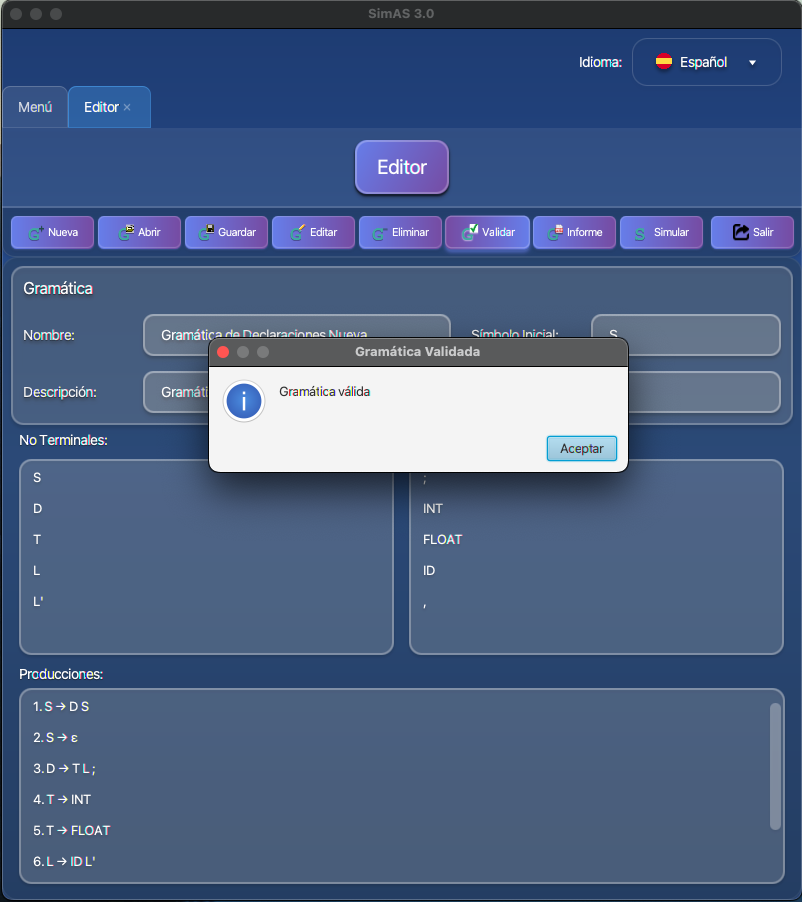
\includegraphics[width=0.9\textwidth]{figuras/editor/validar.png}
    \caption{Validación exitosa de la gramática}
    \label{fig:validar_correcta}
\end{figure}

\subsection{Validación con errores}

Cuando la gramática contiene errores, se muestra la interfaz de la figura \ref{fig:validar_incorrecta}.

\needspace{8cm}
\begin{figure}[H]
    \centering
    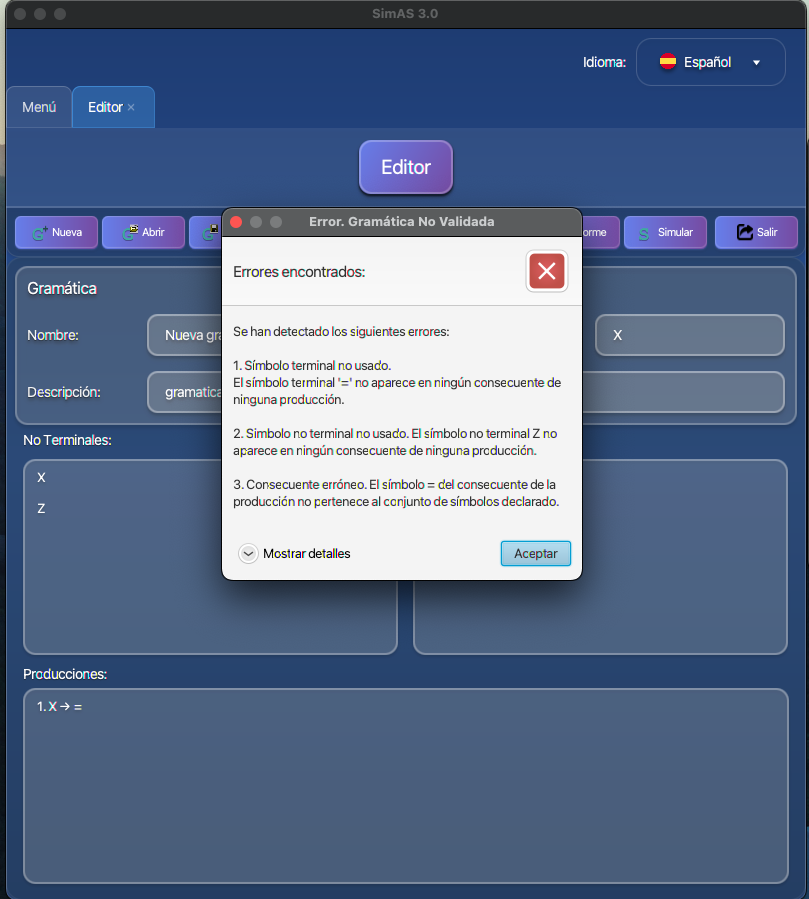
\includegraphics[width=0.9\textwidth]{figuras/editor/validar_incorrecta.png}
    \caption{Validación con errores en la gramática}
    \label{fig:validar_incorrecta}
\end{figure}

\subsection{Tipos de errores detectados}

El sistema de validación detecta los siguientes tipos de errores:

\begin{itemize}
    \item \textbf{Símbolos duplicados}: cuando se define el mismo símbolo múltiples veces.
    \item \textbf{Referencias no definidas}: cuando se usa un símbolo que no ha sido definido.
    \item \textbf{Producciones mal formadas}: cuando las producciones no siguen el formato correcto.
    \item \textbf{Símbolo inicial no definido}: cuando el símbolo inicial no está en la lista de no terminales.
\end{itemize}

\subsection{Ejemplo de error: símbolo duplicado}

La figura \ref{fig:simbolo_duplicado} muestra un ejemplo de error por símbolo duplicado.

\needspace{8cm}
\begin{figure}[H]
    \centering
    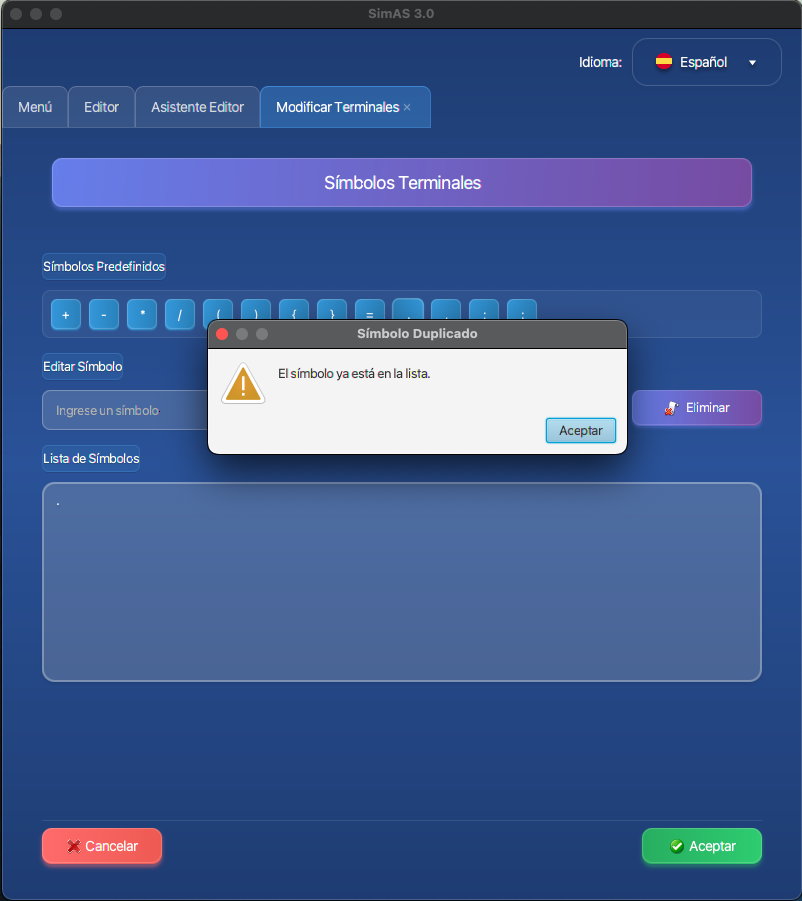
\includegraphics[width=0.9\textwidth]{figuras/editor/simbolo_duplicado.png}
    \caption{Ejemplo de error: símbolo duplicado}
    \label{fig:simbolo_duplicado}
\end{figure}

\subsection{Corrección de errores}

Para corregir errores de validación:

\begin{enumerate}
    \item Revise los mensajes de error mostrados en la interfaz.
    \item Identifique el tipo de error y su ubicación.
    \item Use el botón \string"Editar\string" para abrir el asistente y corregir los errores.
    \item Vuelva a validar la gramática hasta que sea correcta.
\end{enumerate}

\section{Integración con el simulador}

El editor está completamente integrado con el simulador de análisis sintáctico, permitiendo una transición fluida entre la creación y la prueba de gramáticas.

\subsection{Transición al simulador}

Para probar una gramática:

\begin{enumerate}
    \item Complete la creación y validación de la gramática en el editor.
    \item Haga clic en el botón \string"Simular\string" en la barra de herramientas.
    \item La gramática se transfiere automáticamente al simulador.
    \item Se abre una nueva pestaña con el simulador.
\end{enumerate}

\subsection{Sincronización de datos}

La integración incluye:

\begin{itemize}
    \item \textbf{Transferencia automática}: la gramática se pasa al simulador sin intervención manual.
    \item \textbf{Estado compartido}: ambos componentes mantienen el mismo estado de la gramática.
    \item \textbf{Navegación fluida}: transición suave entre editor y simulador.
\end{itemize}

\section{Resolución de problemas}

Esta sección aborda los problemas más comunes que pueden surgir al usar el editor.

\subsection{Problemas de validación}

Si la gramática no pasa la validación:

\begin{enumerate}
    \item Revise los mensajes de error mostrados en la interfaz.
    \item Verifique que todos los símbolos estén correctamente definidos.
    \item Asegúrese de que las producciones sigan el formato correcto.
    \item Use el botón \string"Editar\string" para corregir los errores identificados.
\end{enumerate}

\subsection{Problemas de archivos}

Para resolver problemas con archivos:

\begin{itemize}
    \item \textbf{Formato de archivo}: asegúrese de que los archivos estén en formato XML válido.
    \item \textbf{Versión}: verifique que esté usando la versión correcta de SimAS 3.0.
    \item \textbf{Caracteres especiales}: evite caracteres no estándar en nombres de símbolos.
    \item \textbf{Encoding}: use codificación UTF-8 para archivos de texto.
\end{itemize}

\section{Conclusión}

El editor de gramáticas de SimAS 3.0 representa una herramienta completa y profesional para la creación y gestión de gramáticas libres de contexto. Su diseño intuitivo, basado en un asistente guiado de 4 pasos, lo convierte en una solución ideal tanto para estudiantes que están aprendiendo los conceptos básicos como para profesionales que requieren herramientas sofisticadas.

El asistente guiado simplifica significativamente el proceso de creación de gramáticas, dividiendo la tarea compleja en pasos manejables: definición de datos, gestión de símbolos, creación de producciones y selección del símbolo inicial. La validación automática para gramáticas cargadas y las creadas o modificadas aseguran la corrección de las gramáticas antes de su uso.

La integración perfecta con el simulador, la gestión robusta de archivos en formato XML, y la capacidad de detectar y corregir errores comunes hacen del editor una herramienta indispensable para cualquier persona que trabaje con gramáticas formales. El enfoque pedagógico del asistente guiado, junto con las funciones de validación y corrección de errores, asegura que la herramienta sea útil en todos los niveles de experiencia.

La capacidad de trabajar con el formato BNF estándar, la gestión eficiente de archivos, y la integración profunda con el resto de la aplicación, posicionan al editor de gramáticas como el componente central de SimAS 3.0, facilitando el aprendizaje y la aplicación práctica de los conceptos de análisis sintáctico descendente predictivo.
